\documentclass[border={-3mm -3mm -3mm -3mm}]{standalone}
\usepackage{tikz}
\usepackage{inconsolata}
\usetikzlibrary{positioning,backgrounds}

\definecolor{bg}{rgb}{1,1,0.9}
\definecolor{node}{rgb}{0.4,0.4,0.3}
\definecolor{edgel}{rgb}{0.7,0.7,0.8}
\definecolor{edged}{rgb}{0.3,0.3,0.4}

\tikzset{
  arrout/.style = {<-,> = latex,pos=0.64}, 
  lab/.style = {fill=bg,font=\ttfamily\bfseries,inner sep=0.5pt},
  arrin/.style = {->,> = latex,pos=0.36},
  entity/.style = {draw,thick,fill=node,node,font=\ttfamily\bfseries,text=bg,circle,inner sep=1pt},
  arr/.style = {edgel,thin},
  arrd/.style = {edged,very thick}
}
\newlength{\hgap}
\setlength{\hgap}{0.2cm}

\begin{document}
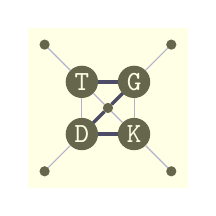
\begin{tikzpicture}[background rectangle/.style={fill=bg}, show background rectangle]
\node[entity] (c) {};

\node[entity,above left=\hgap of c] (t) {T}
  edge[arr] (c);
  
\node[entity,above right=\hgap of c] (g) {G}
  edge[arrd] (c)
  edge[arrd] (t);
  
\node[entity,below left=\hgap of c] (d) {D}
  edge[arrd] (c)
  edge[arr] (t);

\node[entity,below right=\hgap of c] (k) {K}
  edge[arr] (c)
  edge[arr] (g)
  edge[arrd] (d);

\node[entity,below right=2\hgap of k] (kc) {}
  edge[arr] (k);

\node[entity,below left=2\hgap of d] (dc) {}
  edge[arr] (d);

\node[entity,above left=2\hgap of t] (tc) {}
  edge[arr] (t);

\node[entity,above right=2\hgap of g] (gc) {}
  edge[arr] (g);

%\node[entity,fill=blue!50!black,right=\hgap of i] (c) {C}
%  edge[arrout] node[lab] {J} (i);
%  
%\node[entity,fill=red,right=\hgap of c] (g) {G}
%  edge[arrout] node[lab] {K} (c)
%  edge[arrin,font=\ttfamily,bend left=55,pos=0.5] node[lab,font=\ttfamily] {21} (i)
%  edge[arrout,bend right=55,pos=0.5] node[lab,font=\ttfamily] {20} (i);
\end{tikzpicture}
\end{document} 